\section{Preliminary Results and Findings}
\label{sec:preliminary_results}

This section presents the results obtained from training a subset of the algorithms discussed in section \ref{subsec:algorithm_selection}. The selected algorithms include five DQN-based methods — DQN, Double DQN, Prioritized Experience Replay, Dueling DQN, and C51 — as well as three policy-based methods: REINFORCE, PPO, and SAC. Soft Actor Critic was preferred to DDPG and TD3 because it can simply be seen as a variation that works with a stochastic policy, but is more easily adapted to a discrete action space.

We first describe necessary modifications to the experiment setup, followed by a detailed analysis of each algorithm's performance and emissions. The results are then compared across different algorithm families.

\subsection{Experiment Setup Adjustments}
\label{subsec:exp_setup_adjustments}
During initial training attempts, some adjustments were required to ensure reliable performance and energy tracking. One key reason for this was that employing CodeCarbon as a (next-)real-time emissions tracking tool significantly slowed down training (by a factor of 20 or more). As a result, we opted to record only total emissions at the end of training rather than tracking them continously. This adjustment allowed us to obtain meaningful comparisons without excessively increasing training time.

In addition to this, on Windows, CodeCarbon's CPU energy tracking relies on the Intel Power Gadget, which has been deprecated for several years. Furthermore, it does not support Intel Performance Counter Monitor (Intel PCM), the official successor to the Power Gadget. In such cases, CodeCarbon switches to a fallback mode, directly quoting from their documentation:
\begin{quoting}
	\begin{itemize}
		\item It will first detect which CPU hardware is currently in use, and then map it to a data source listing 2000+ Intel and AMD CPUs and their corresponding thermal design powers (TDPs).
		
		\item If the CPU is not found in the data source, a global constant will be applied. CodeCarbon assumes that 50\% of the TDP will be the average power consumption to make this approximation.
		
		\item We could not find any good resource showing statistical relationships between TDP and average power, so we empirically tested that 50\% is a decent approximation.
	\end{itemize}
\end{quoting}

This approach should provide reasonable estimates for our project, since most of the workload is on the GPU, while the rest is mostly constant across the algorithms (like the environment simulations). This being said, one instance where this limitation may have had an impact is in tracking the Proximal Policy Optimization (PPO) algorithm, that employs a relatively small neural network but requires more CPU and RAM processing, the latter also explicitly stated to not be tracked satisfactorily.

Moreover, wandb collect systems data, but it also, while collecting kwh for the gpu, does not for cpu and ram, so we have to make do with what we have

Additionally, Weights \& Biases collects system data during training, and while it tracks GPU energy consumption in kWh, it also does not do the same for CPU and RAM. As a result, while we can obtain excellent emissions estimates for the GPU, CPU and RAM energy tracking remains imprecise due to the aforementioned limitations. Consequently, energy consumption analyses must be interpreted with an understanding of these constraints.

\subsection{DQN-Based Algorithms}
We present results for five different DQN-based algorithms, including baseline DQN and its extensions. Each algorithm is analyzed individually before an overall comparison.

\subsubsection{DQN (Baseline)}
\label{subsubsec:dqn}

In our benchmark, \emph{Deep Q-Network (DQN)} serves as the baseline algorithm against which we compare more advanced DQN variants and policy gradient methods. We trained DQN on the selected eight Atari games, running four distinct seeds per game for a total of 32 runs. Table~\ref{tab:dqn-hyperparams} summarizes the main hyperparameters used; the total number of training steps was \num{100000} in each run.

\paragraph{Hyperparameters.}
\begin{table}[htb]
	\centering
	\begin{tabular}{l l}
		\toprule
		\textbf{Parameter} & \textbf{Value} \\
		\midrule
		\texttt{learning\_rate} & \num{1e-4} \\
		\texttt{buffer\_size} & \num{10000} \\
		\texttt{batch\_size} & \num{32} \\
		\texttt{target\_network\_frequency} & \num{1000} \\
		\texttt{exploration\_fraction} & \num{0.1} \\
		\texttt{start\_e}, \texttt{end\_e} & \num{1.0} $\to$ \num{0.01} \\
		\texttt{learning\_starts} & \num{1000} \\
		\texttt{train\_frequency} & \num{4} \\
		\bottomrule
	\end{tabular}
	\caption{Key hyperparameters for the DQN baseline. 
		All runs used a discount factor $\gamma = 0.99$,
		one environment (\texttt{num\_envs}=1), 
		and \texttt{cuda} enabled.}
	\label{tab:dqn-hyperparams}
\end{table}

\paragraph{Training Dynamics.}
Figure~\ref{fig:dqn_episodic_length} shows the \emph{episodic length} during training, aggregated over the 32 runs via linear interpolation onto a common step axis. We observe that the \emph{mean} episode length hovers around 3500--4000 steps for most of training, with substantial variability among runs (up to 8000 steps in the most extreme cases). In some runs, episodes became quite short, indicating early terminations and resulting in the large min--max envelope.

Figure~\ref{fig:dqn_episodic_return} presents the \emph{episodic return} curves. The mean performance remains slightly below zero for most of the training, reflecting the difficulty of some games given only \num{100000} steps of interaction. In a few runs, we observe short-lived spikes in performance, but overall there is high variance (the min--max band ranges from about $-10$ to $+4$). These preliminary results suggest that DQN can struggle to achieve consistently positive returns in the chosen set of Atari games within 100k steps.

\paragraph{Loss and Value Estimates.}
To further diagnose training behavior, Figure~\ref{fig:dqn_q_values} shows the evolution of the estimated \emph{Q-values} over training. Notably, the mean $Q$ grows from near zero to around $4$ or $5$ by step \num{100000}, but with large min--max variability (some runs estimate $Q$-values above $10$, while others stay near $0$). Meanwhile, the \emph{TD loss} (Figure~\ref{fig:dqn_td_loss}) starts near zero and steadily increases in many runs, peaking in some seeds above $1.0$ or even $3.0$ toward the end of training. These indicators suggest that DQN’s learning process under these hyperparameters and time horizons remains quite unstable, highlighting the challenges of sample efficiency in a short \num{100000}-step regime.

\paragraph{Energy Consumption.}
Table~\ref{tab:dqn-emissions} shows the average carbon emissions for DQN over the eight games (four seeds each). On average, \textbf{0.00647 kg} of CO\textsubscript{2} was emitted per run (with a standard deviation of $0.00026$).%
\footnote{Exact units can vary depending on CodeCarbon’s tracking settings; here we report total kg CO\textsubscript{2} equivalent for each run.}
While this raw number is relatively small, it is still a meaningful measurement in comparing algorithms’ resource usage—particularly if scaled up to longer training horizons or larger runs.

\begin{table}[htb]
	\centering
	\begin{tabular}{lcccccccc}
		\toprule
		\textbf{Algorithm} & \textbf{mean} & \textbf{std} & \textbf{median} & \textbf{q25} & \textbf{q75} & \textbf{min} & \textbf{max} & \textbf{iqmean}\\
		\midrule
		DQN & 0.00647 & 0.00026 & 0.00634 & 0.00630 & 0.00658 & 0.00616 & 0.00699 & 0.00637 \\
		\bottomrule
	\end{tabular}
	\caption{Carbon emissions for DQN (\emph{kg CO\textsubscript{2} eq.}) aggregated across 32 runs.}
	\label{tab:dqn-emissions}
\end{table}

\paragraph{Observations}
Overall, DQN shows moderate performance with high variance and relatively low returns within the \num{100000}-step constraint. The Q-values and TD loss reveal ongoing instability, suggesting that more advanced extensions or longer training might be necessary to achieve robust performance on these Atari tasks. In terms of energy footprint, DQN remains relatively lightweight in absolute terms, though differences may become more pronounced when compared with other algorithms (Section~\ref{subsubsec:ddqn} and beyond) or when scaled to larger training budgets.

\begin{figure}[htbp]
	\centering
	% Replace with your actual figure command or path:
	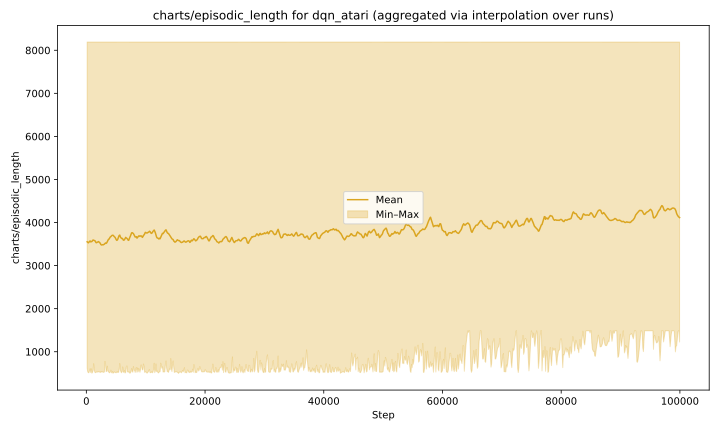
\includegraphics[width=0.6\textwidth]{figures/charts_episodic_length_dqn_atari.png}
	\caption{DQN episodic length (\texttt{charts/episodic\_length}), showing mean (line) and min--max band (shaded).}
	\label{fig:dqn_episodic_length}
\end{figure}

\begin{figure}[htbp]
	\centering
	% Replace with your actual figure command or path:
	\includegraphics[width=0.6\textwidth]{figures/charts_episodic_return_dqn_atari.png}
	\caption{DQN episodic return (\texttt{charts/episodic\_return}), showing mean (line) and min--max band (shaded).}
	\label{fig:dqn_episodic_return}
\end{figure}

\begin{figure}[htbp]
	\centering
	% Replace with your actual figure command or path:
	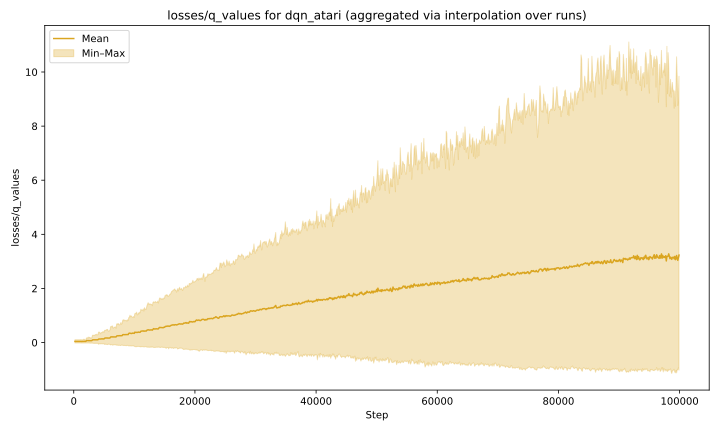
\includegraphics[width=0.6\textwidth]{figures/losses_q_values_dqn_atari.png}
	\caption{Estimated Q-values (\texttt{losses/q\_values}) for DQN, showing mean and min--max across runs.}
	\label{fig:dqn_q_values}
\end{figure}

\begin{figure}[htbp]
	\centering
	% Replace with your actual figure command or path:
	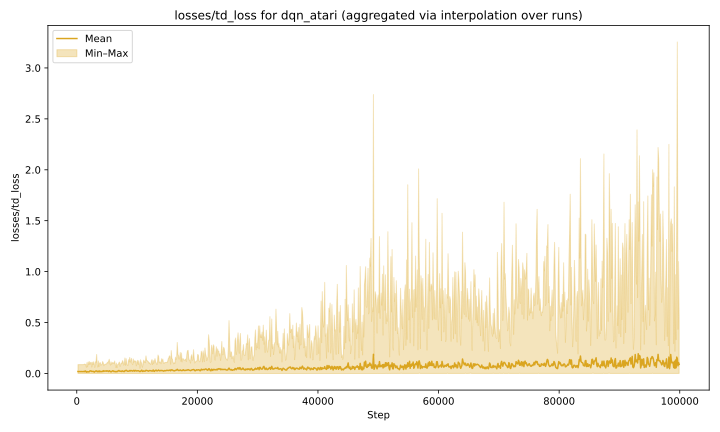
\includegraphics[width=0.6\textwidth]{figures/losses_td_loss_dqn_atari.png}
	\caption{TD loss (\texttt{losses/td\_loss}) for DQN, illustrating the growing variance across runs.}
	\label{fig:dqn_td_loss}
\end{figure}

\noindent In the following subsections, we examine how enhancements such as Double DQN and Prioritized Experience Replay improve upon this baseline in terms of both performance and energy consumption.


\subsubsection{Double DQN}
\label{subsubsec:ddqn}
\begin{itemize}
	\item Differences from baseline DQN.
	\item Training execution and results.
	\item \textbf{Comparison with DQN:} Score improvement, energy trade-offs.
\end{itemize}
Differences from baseline DQN.
Training execution and results.
Comparison with DQN in terms of score, stability, and energy efficiency.


\subsubsection{Prioritized Experience Replay}
\begin{itemize}
	\item How prioritization improved learning efficiency.
	\item Energy-performance trade-off compared to DQN and Double DQN.
\end{itemize}
Comparison with DQN and Double DQN.
Did it lead to better sample efficiency?
Energy consumption comparison.


\subsubsection{Dueling DQN}
\begin{itemize}
	\item Did dueling networks reduce variance?
	\item Performance and energy efficiency compared to other DQN methods.
\end{itemize}
Impact on stability.
Did it reduce variance in Q-value estimates?
Performance and energy trade-offs.


\subsubsection{C51 (Categorical DQN)}
\begin{itemize}
	\item Impact of distributional reinforcement learning.
	\item Did C51 improve sample efficiency?
\end{itemize}
Did distributional learning improve performance?
Energy efficiency vs. performance trade-off.


\subsection{Overall Comparison of DQN-Based Algorithms}
\begin{itemize}
	\item Graphs comparing all DQN-based methods.
	\item Summary table with:
	\begin{itemize}
		\item Final performance scores per game.
		\item Total training duration.
		\item Energy consumption.
	\end{itemize}
	\item Discussion: Which method offers the best balance between efficiency and performance?
\end{itemize}
Graphs comparing all 5 DQN-based algorithms on the same scale.
Tables summarizing:
Performance (average final score per game).
Training duration.
Total energy consumption.
Key takeaways: Which is the best energy-performance trade-off?

\subsection{Policy-Based Algorithms}
This section presents results for the three policy gradient methods.

\subsubsection{REINFORCE}
\begin{itemize}
	\item Training execution and stability.
	\item Performance scores and energy consumption.
\end{itemize}
Training execution.
Stability of policy gradient training.
Final scores and emissions.


\subsubsection{PPO (Proximal Policy Optimization)}
\begin{itemize}
	\item Effect of clipping on training stability.
	\item Performance vs. REINFORCE.
\end{itemize}
Did clipping help stabilize training?
Efficiency compared to REINFORCE.


\subsubsection{SAC (Soft Actor-Critic)}
\label{subsubsec:sac}
\begin{itemize}
	\item Impact of entropy regularization.
	\item Energy efficiency compared to PPO and REINFORCE.
\end{itemize}
How did the entropy regularization affect performance?
Energy trade-offs (is SAC more expensive to train?).


\subsection{Overall Comparison of Policy-Based Algorithms}
\begin{itemize}
	\item Graphs comparing all policy-based methods.
	\item Which method achieved better stability?
	\item Summary of trade-offs between energy consumption and performance.
\end{itemize}
Graphs comparing policy-based methods.
Which is more stable? Which is more efficient?
Final takeaway: Did one clearly outperform the others in both energy efficiency and reward?


\subsection{Cross-Category Comparison: DQN vs. Policy Gradient}
\begin{itemize}
	\item Which family was more energy-efficient?
	\item Graphs comparing the best-performing models from each category.
	\item Conclusion: Do policy-based methods require more energy but provide better sample efficiency?
\end{itemize}
Which family is generally more energy-efficient?
Graphs comparing best DQN-based vs. best policy-based model.
Final summary of the findings.